\usetikzlibrary{3d,decorations.text,shapes.arrows,positioning,fit,backgrounds}
\tikzset{pics/fake box/.style args={% #1=color, #2=x dimension, #3=y dimension, #4=z dimension
#1 with dimensions #2 and #3 and #4}{
code={
\draw[gray,ultra thin,fill=#1]  (0,0,0) coordinate(-front-bottom-left) to
++ (0,#3,0) coordinate(-front-top-right) --++
(#2,0,0) coordinate(-front-top-right) --++ (0,-#3,0) 
coordinate(-front-bottom-right) -- cycle;
\draw[gray,ultra thin,fill=#1] (0,#3,0)  --++ 
 (0,0,#4) coordinate(-back-top-left) --++ (#2,0,0) 
 coordinate(-back-top-right) --++ (0,0,-#4)  -- cycle;
\draw[gray,ultra thin,fill=#1!80!black] (#2,0,0) --++ (0,0,#4) coordinate(-back-bottom-right)
--++ (0,#3,0) --++ (0,0,-#4) -- cycle;
\path[gray,decorate,decoration={text effects along path,text={CONV}}] (#2/2,{2+(#3-2)/2},0) -- (#2/2,0,0);
}
}}
% from https://tex.stackexchange.com/a/52856/121799
\tikzset{circle dotted/.style={dash pattern=on .05mm off 2mm,
                                         line cap=round}}

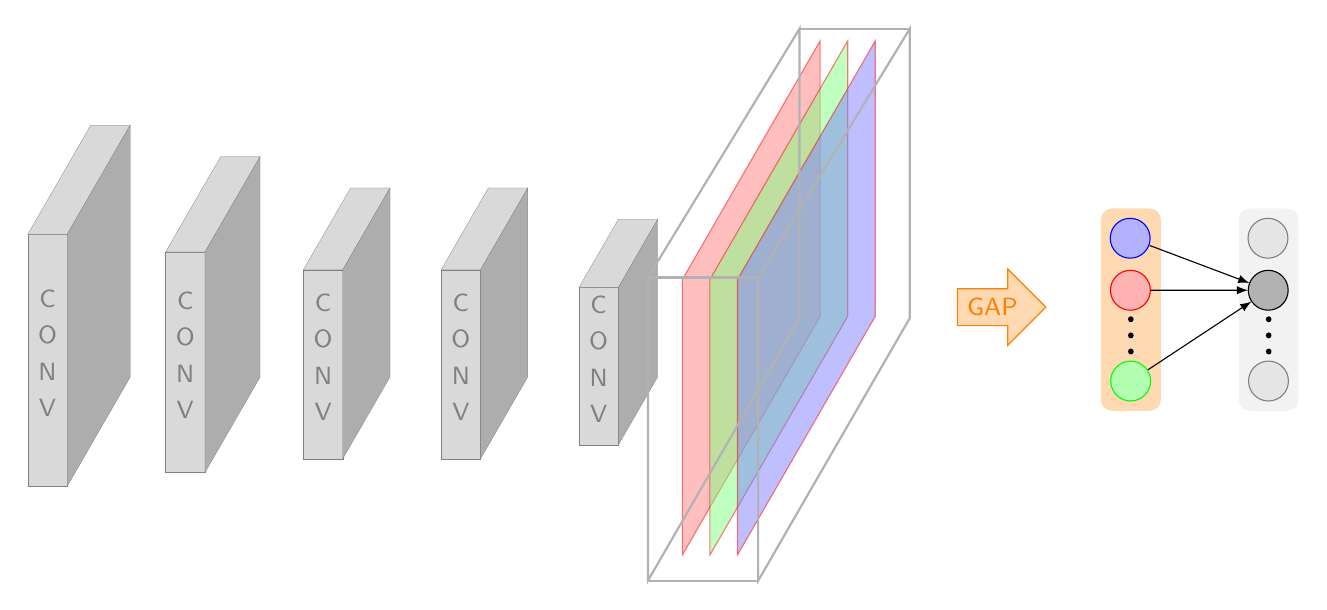
\begin{tikzpicture}[x={(1,0)},y={(0,1)},z={({cos(60)},{sin(60)})},
font=\sffamily\small,scale=1.75]
%
% comment these out if you want to see where the axes point to
% \draw[-latex] (0,0,0) -- (3,0,0) node[below]{$x$};
% \draw[-latex] (0,0,0) -- (0,3,0) node[left]{$y$};
% \draw[-latex] (0,0,0) -- (0,0,3) node[below]{$z$};
% a plane
\foreach \X [count=\Y] in {1.6,1.4,1.2,1.2,1}
{
\draw pic (box1-\Y) at (\Y,-\X/2,0) {fake box=white!70!gray with dimensions 0.5 and {2*\X} and 1*\X};
}

\foreach \X/\Col in {6.5/red,6.7/green,6.9/blue}
{\draw[canvas is yz plane at x = \X, transform shape, draw = red, fill =
\Col!50!white, opacity = 0.5] (0,0.5) rectangle (2,-1.5);}
\draw[gray!60,thick] (6.3,-0.1,-1.6) coordinate (1-1) -- (6.3,-0.1,0.6) coordinate (1-2) -- (6.3,2.,0.6) coordinate (1-3) -- (6.3,2.1,-1.6) coordinate (1-4) -- cycle;
\draw[gray!60,thick] (7.1,-0.1,-1.6) coordinate (2-1) -- (7.1,-0.1,0.6) coordinate (2-2) -- (7.1,2.,0.6) coordinate (2-3) -- (7.1,2.1,-1.6) coordinate (2-4) -- cycle;
\foreach \X in {4,1,3}
{\draw[gray!60,thick] (1-\X) -- (2-\X);}
%
\node[draw,single arrow, orange,fill=orange!30] at (8,0.5,0) {GAP};
\node[circle,draw,blue,fill=blue!30] (A1) at (9,1,0) {~~~};
\node[circle,draw,red,fill=red!30,below=4pt of A1] (A2) {~~~};
\node[circle,draw,green,fill=green!30,below=18pt of A2] (A3) {~~~};
\draw[circle dotted, line width=2pt,shorten <=3pt] (A2) -- (A3);
\node[circle,draw,gray,fill=gray!20] (B1) at (10,1,0) {~~~};
\node[circle,draw,fill=gray!60,below=4pt of B1] (B2) {~~~};
\node[circle,draw,gray,fill=gray!20,below=18pt of B2] (B3) {~~~};
\draw[circle dotted, line width=2pt,shorten <=3pt] (B2) -- (B3);
\begin{scope}[on background layer]
\node[orange,thick,rounded corners,fill=orange!30,fit=(A1) (A3)]{};
\node[gray,thick,rounded corners,fill=gray!10,fit=(B1) (B3)]{};
\end{scope}
\foreach \X in {1,2,3}
{\draw[-latex] (A\X) -- (B2);}
\end{tikzpicture}